\documentclass[11pt]{article}
\usepackage[margin=1in]{geometry}
\usepackage{amsmath,amssymb,graphicx,listings,xcolor,float}
\usepackage{enumitem}

\lstset{
  language=Matlab,
  basicstyle=\small\ttfamily,
  keywordstyle=\color{blue},
  commentstyle=\color{green!50!black},
  stringstyle=\color{red},
  numbers=left,
  numberstyle=\tiny\color{gray},
  breaklines=true,
  frame=single,
  tabsize=4
}

\title{MATH 543 -- Homework 5}
\author{Parham Khodadi}
\date{}

\begin{document}
\maketitle

%% ============================================================
\section*{Problem 12.3 -- Trefethen \& Bau}
%% ============================================================

The goal of this problem is to explore some properties of random matrices. Your job is to be a laboratory scientist, performing experiments that lead to conjectures and more refined experiments. Do not try to prove anything. Do produce well-designed plots, which are worth a thousand numbers.

Define a random matrix to be an $m \times m$ matrix whose entries are independent samples from the real normal distribution with mean zero and standard deviation $\sqrt{m}$ --- In MATLAB, 
\newline \texttt{A = randn(m,m)/sqrt(m)} --- the factor $\sqrt{m}$ is introduced to make the limiting behavior clean as $m \rightarrow \infty$.

\begin{enumerate}[label=\Alph*.]
    \item What do the eigenvalues of a random matrix look like? What happens, say, if you take 100 random matrices and superimpose all their eigenvalues in a single plot? If you do this for m = 8, 16, 32, 64,..., what pattern is suggested? How does the spectral radius $\rho(A)$ (see Exercise 3.2) behave as $m \rightarrow \infty$?
    \item What about norms? How does the 2-norm of a random matrix behave as $m \rightarrow \infty$? Of course, we must have $\rho(A)<||A||$ (see Exercise 3.2). Does this inequality appear to approach an equality as $m \rightarrow \infty$?
    \item What about condition numbers—or more simply, the smallest singular value $\sigma_{min}$? Even for fixed $m$ this question is interesting. What proportions of random matrices in $\mathbb{R}^{m \times m}$ seem to have $\sigma_{min}<2^{-1},2^{-2},2^{-3},...$? In other words, what does the tail of the probability distribution of smallest singular values look like? How does the scale of all this change with $m$?
\end{enumerate}


%% ============================================================
\newpage
\section*{Part A.}
%% ============================================================
\begin{figure}[H]
    \centering
    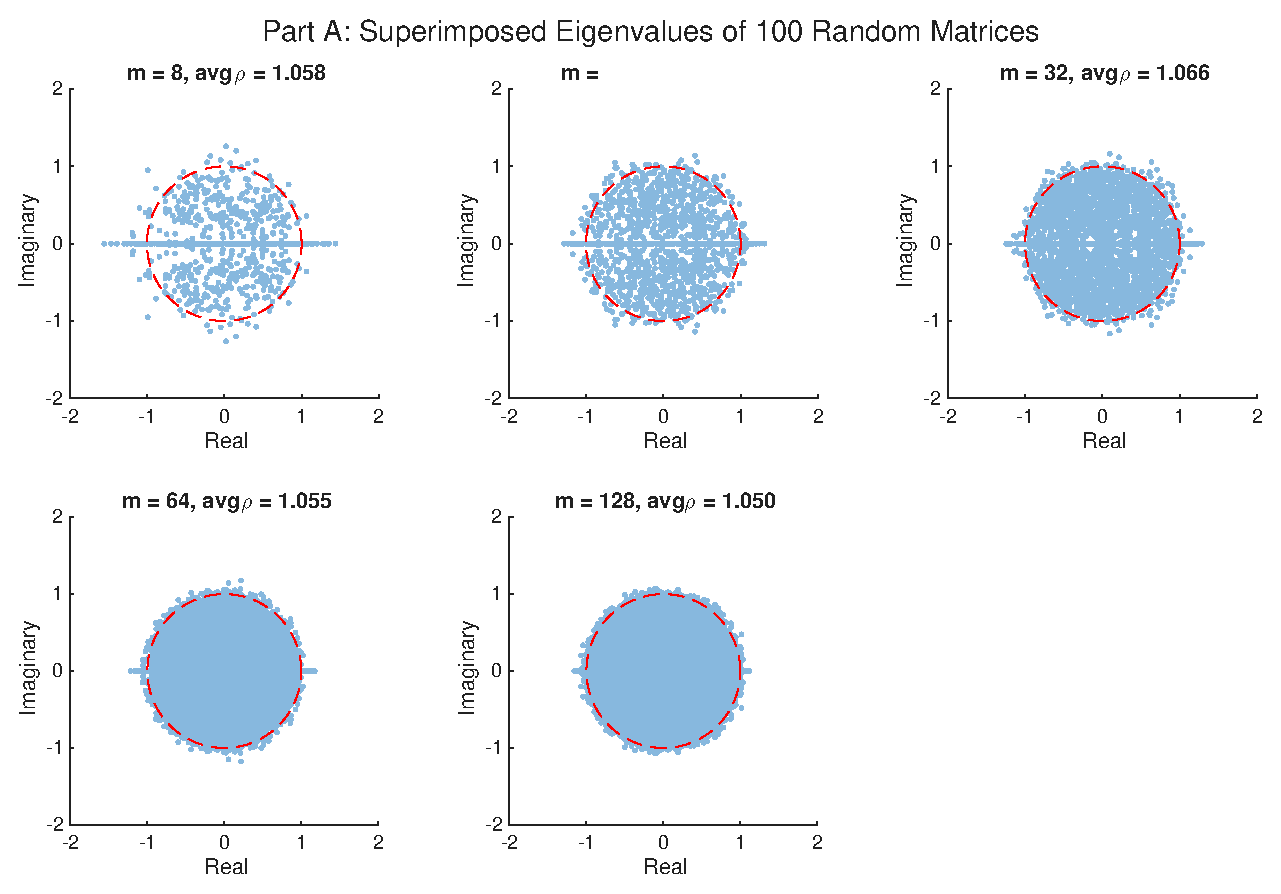
\includegraphics[width=1\linewidth]{Figures/PartA_Eigenvalues.eps}
    \caption{For some reason, LaTeX is having trouble loading the second graph's title. It should read: $m = 16, \rho_{avg} = 1.052$.}
    \label{fig:A}
\end{figure}

My MATLAB code (found in the Appendix) generated Figure \ref{fig:A}. This figure shows that the eigenvalues of random matrices superimposed on the complex plane fall into a roughly uniform circular distribution. As the matrix size $m$ increases, this circular "blob" becomes more dense. This increase in density also makes its outer boundary much sharper.

The red dashed unit circle (radius of 1) perfectly bounds the distribution. As $m \rightarrow \infty$, $\rho \rightarrow 1$. The third graph being a statistical outlier, where the $\rho$ increases rather than decrease towards 1.





%% ============================================================
\newpage
\section*{Part B.}
%% ============================================================
\begin{figure}[H]
    \centering
    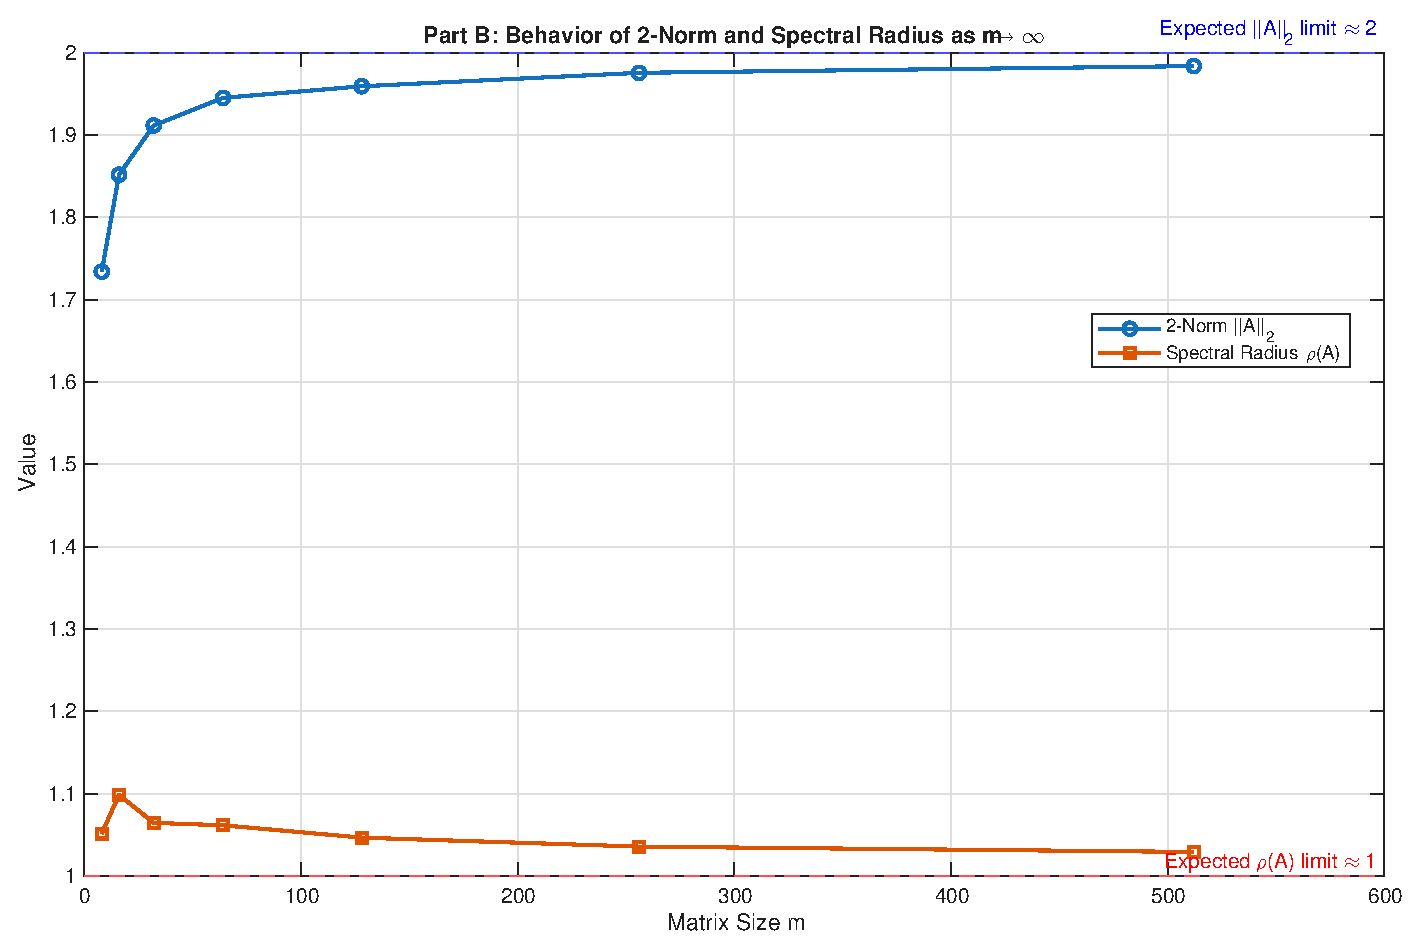
\includegraphics[width=1\linewidth]{Figures/PartB_Norm_Rho.eps}
    \caption{It may be hard to tell, but there exists a blue dashed line at $y=2$ representing the expected value for the 2-norm limit.}
    \label{fig:B}
\end{figure}

My MATLAB code (found in the Appendix) generated Figure \ref{fig:B}. In this figure, you can see that the 2-norm of the random matrix $A$ rapidly parabollically approaches the asymptote of 2. In other words: As $m \rightarrow \infty$, $||A||_2 \rightarrow 2$. At the same time, the spectral radius approaches 1. In other words: As $m \rightarrow \infty$, $\rho(A) \rightarrow 1$.

This graph also answers the question of whether the fundamental inequality $\rho(A) \le ||A||_2$ approaches equality with increasing $m$. Clearly, it does not as $\rho(A) \rightarrow 1$, it remains less than $||A||_2 \rightarrow 2$.


%% ============================================================
\newpage
\section*{Part C.}
%% ============================================================
\begin{figure}[H]
    \centering
    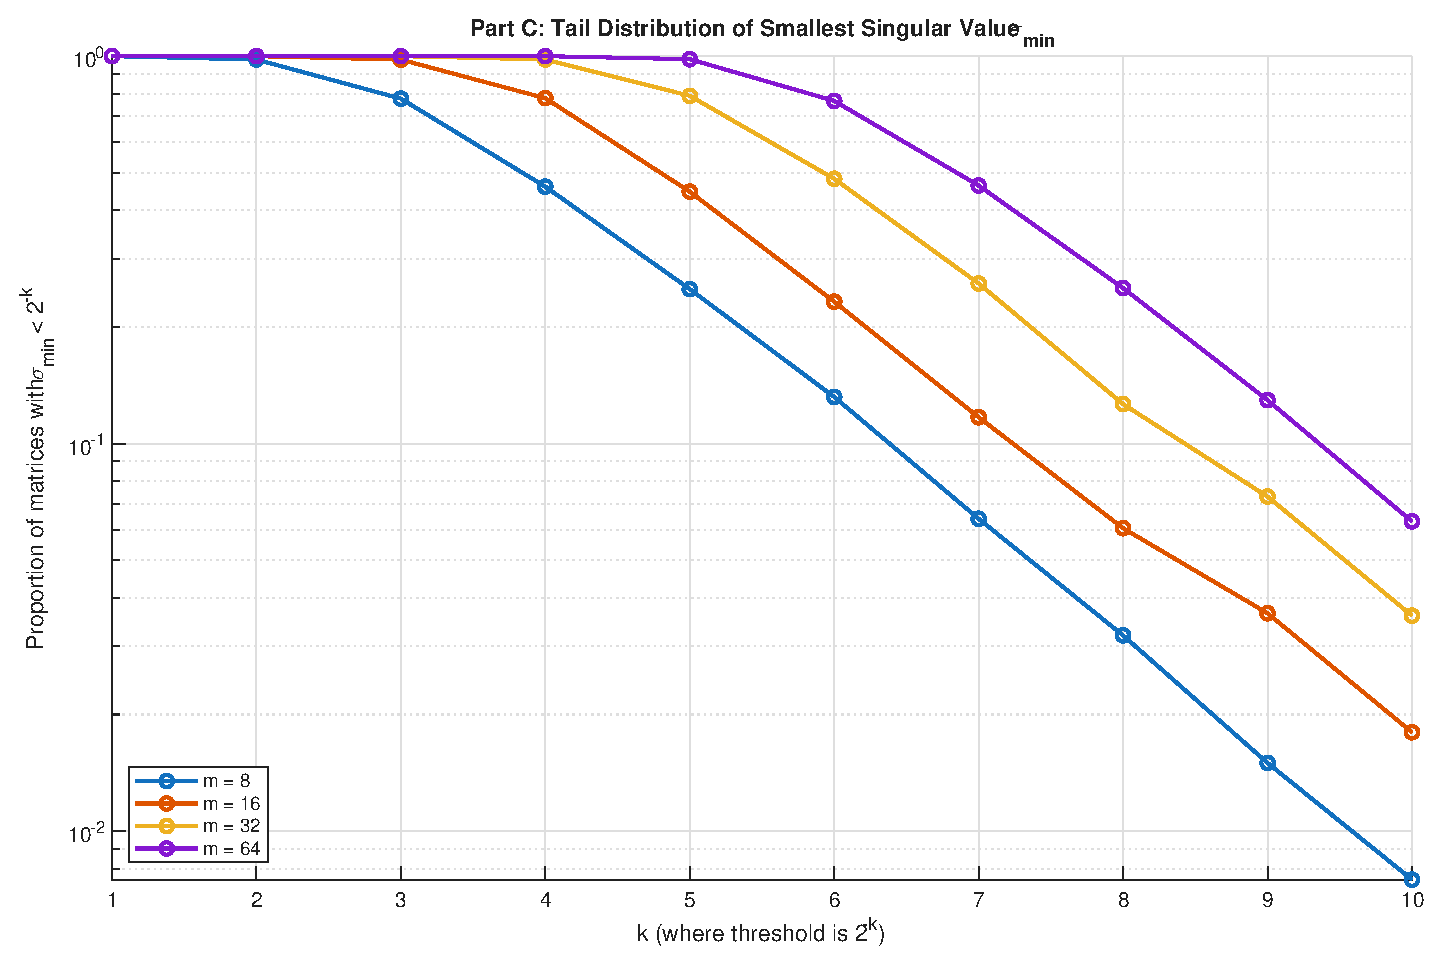
\includegraphics[width=1\linewidth]{Figures/PartC_SigmaMin.eps}
    \caption{Enter Caption}
    \label{fig:C}
\end{figure}

My MATLAB code (found in the Appendix) generated Figure \ref{fig:C}. Because the y-axis is on a logarithmic scale, the straight, parallel lines for higher values of $k$ (roughly $k \geq 3$) indicate a power-law relationship. Since I plotted against $k$ (where the threshold is $2^{-k}$), the linear drop-off confirms that the probability of finding a smallest singular value $\sigma_{\min} < \epsilon$ is directly proportional to $\epsilon$.

Look at the vertical spacing between the lines. For any given $k$, the proportion is higher for larger $m$. If you compare $m=8$ to $m=64$ (an $8\times$ increase in size), the proportion line shifts up by roughly a factor of $8$. This suggests that the probability of drawing an ill-conditioned random matrix increases linearly with the matrix dimension $m$.


%% ============================================================
\newpage
\section*{Appendix: MATLAB Code}
%% ============================================================

\lstinputlisting{HW5.m}

\end{document}